% =============================================================================
% Visual one-page abstract for Paper 5a
% =============================================================================

\documentclass[9pt, letterpaper, landscape]{extarticle}

\usepackage[T1]{fontenc}
\usepackage[utf8]{inputenc}
\usepackage[margin=0.3in]{geometry}
\usepackage{amsmath, amssymb}
\usepackage{graphicx}
\usepackage{xcolor}
\usepackage{booktabs}
\usepackage{tcolorbox}
\usepackage[hidelinks]{hyperref}
\usepackage{microtype}

\usepackage{ifxetex}
\ifxetex
  \usepackage{fontspec}
  \setmainfont{Charter}[Numbers=OldStyle]
\fi

\definecolor{INK}{HTML}{1d1d1d}
\definecolor{RUST}{HTML}{B5482A}
\definecolor{SAGE}{HTML}{4C7066}
\definecolor{GOLD}{HTML}{C28B25}
\definecolor{VIOLET}{HTML}{5E4F7A}
\definecolor{DIM}{HTML}{7a7a7a}

\pagestyle{empty}
\setlength{\parindent}{0pt}
\setlength{\parskip}{2pt}

\begin{document}

\begin{center}
{\large\bfseries The Untaken Limit:} A Pole at $\theta = -2$ in the Head-Mayer Closed Form for Intra-National Distance\\
{\footnotesize Ian T. Helfrich \;{\color{DIM}\textbar}\; Georgia Tech \;{\color{DIM}\textbar}\; \today \;{\color{DIM}\textbar}\; \texttt{github.com/ihelfrich/paper5-effective-distance}}
\end{center}

\vspace{-4pt}

\noindent\begin{minipage}[t]{0.36\textwidth}
{\color{RUST}\rule{\textwidth}{0.6pt}}\\
\textbf{\color{RUST}The setup.}
Every gravity regression since 2005 uses CEPII's \texttt{distw\_harmonic} as
the intra-national distance. CEPII constructs it from the Head-Mayer (2002)
CES integral $d_{ii}(\theta) = (2/(\theta+2))^{1/\theta} R$, evaluated at
$\theta = -1$. Mayer-Zignago (2011) justify $\theta = -1$ as ``the usual
coefficient estimated from gravity models''---the reduced-form regression
slope, not the structural CES integration parameter $\theta = \delta(1-\sigma)$,
which for $\sigma \in [4,8]$ and $\delta = 1$ falls in $[-7, -3]$.\\[3pt]

{\color{RUST}\rule{\textwidth}{0.6pt}}\\
\textbf{\color{RUST}The pole.}
The closed form has a pole at $\theta = -2$: complex-valued for $\theta < -2$.
The underlying integral $\int_0^R r^{\theta+1}\, dr$ diverges in 2D for
$\theta \leq -2$. \textbf{Structurally consistent values fall entirely
below the pole.}\\[3pt]

\begin{tcolorbox}[colback=GOLD!5, colframe=GOLD, boxrule=0.5pt,
  arc=2pt, left=3pt, right=3pt, top=2pt, bottom=2pt]
{\footnotesize\bfseries Closed form at $R = 1000$ km:}\\[1pt]
{\footnotesize
$\theta = +1$:\; $667$ km (arithmetic mean)\\
$\theta = -1$:\; $500$ km\; {\color{RUST}\textbf{(CEPII)}}\\
$\theta = -1.99$:\; $9.5$ km (near pole)\\
$\theta = -2$:\; \textbf{\color{RUST}POLE}\\
$\theta = -3, -5, -7$:\; \textbf{\color{RUST}complex} (gravity-consistent)}
\end{tcolorbox}

{\color{RUST}\rule{\textwidth}{0.6pt}}\\
\textbf{\color{RUST}The consequence.}
At gravity-consistent $\sigma$, $d_{ii}$ has no fixed value. The
home-bias coefficient inherits the regularization choice $d_{\min}$:
from $-2.92$ (multiplier $0.05\times$) at fine resolution to $+2.13$
(multiplier $8.4\times$, the canonical McCallum finding) at the CEPII
baseline. \textbf{The border puzzle lives inside the measurement window.}

\end{minipage}
\hfill
\begin{minipage}[t]{0.62\textwidth}

\centering
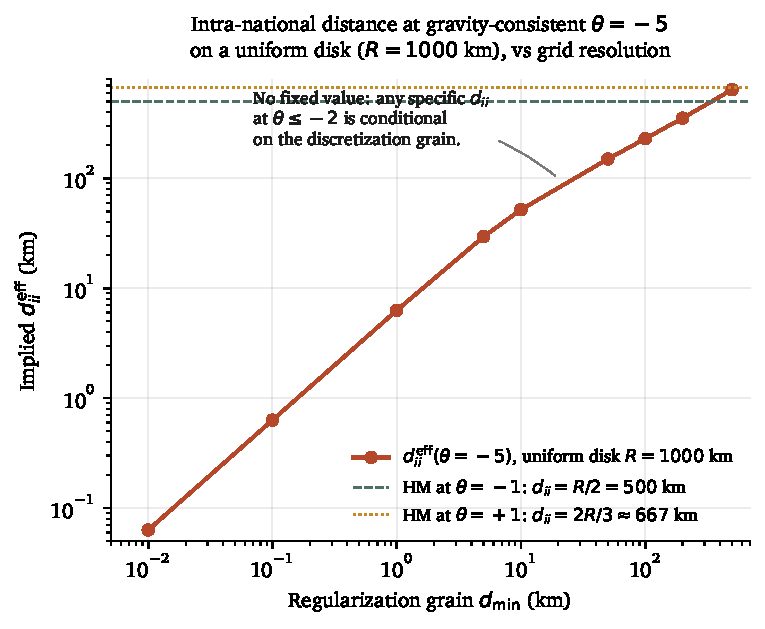
\includegraphics[width=0.7\textwidth]{figures/fig1_regularization_curve.pdf}\\[1pt]
{\footnotesize\itshape Fig 1. Implied $d_{ii}^{\rm eff}(\theta=-5)$ on a
uniform disk: two-order-of-magnitude span from the regularization grain alone.}

\vspace{4pt}

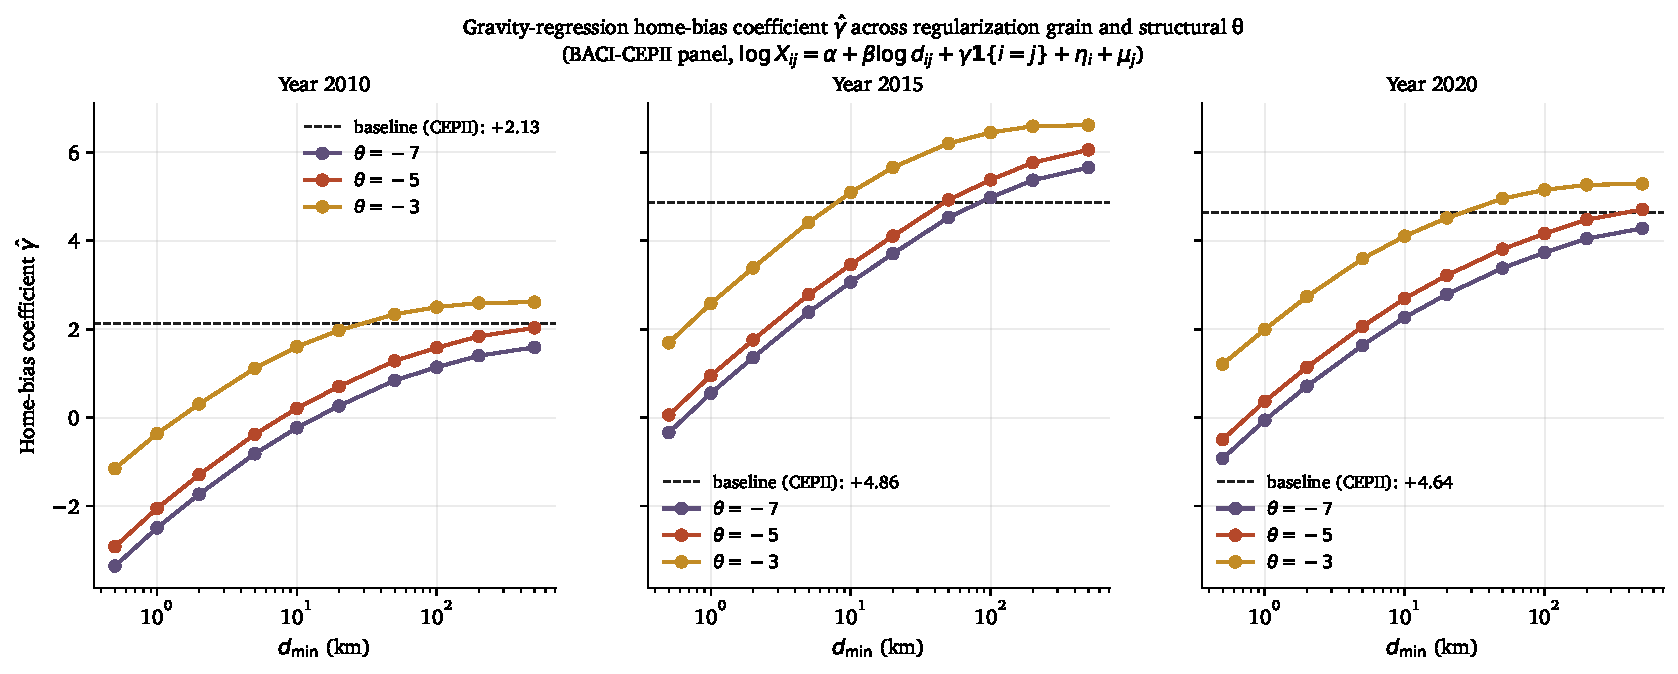
\includegraphics[width=0.95\textwidth]{figures/fig2_home_bias_vs_dmin.pdf}\\[1pt]
{\footnotesize\itshape Fig 2. Home-bias coefficient $\hat\gamma$ vs the
regularization grain, by year and structural $\theta$. CEPII baseline
(dashed) at the high-$d_{\min}$ end; sign-flip threshold between 1 and 5 km.}

\end{minipage}

\vspace{-4pt}

\begin{tcolorbox}[colback=SAGE!5, colframe=SAGE, boxrule=0.5pt,
  arc=2pt, left=6pt, right=6pt, top=3pt, bottom=3pt]
\textbf{\color{SAGE}Takeaway.}
Border-puzzle multipliers have been reported as structural objects rather
than as conditional on a regularization. A $10\times$ multiplier at
$d_{\min} = 100$ km and a $5\times$ multiplier at $d_{\min} = 10$ km are
not contradictions; they are the same regression conditional on different
regularizations. The structurally consistent procedure is to acknowledge
that $d_{ii}$ is not a well-defined object at gravity-consistent
$\sigma$, and to estimate the model in a way that does not pin $d_{ii}$
to a single number.
\end{tcolorbox}

\end{document}
